\chapter{Architecture and Implementation}
\label{ch:architecture-and-implementation}

  \section{Scheduling and Adaptation Approach}
  \label{sec:scheduling-and-adaptation-approach-architecture}

    \subsection{Scheduling and Adaptation Functional Architecture}
    The architecture of the integrated \SAA{} scheduling and adaptation tool consists of five components, displayed in Figure~\ref{fig:data-cloud-architecture}.

    \begin{figure}
        \centering
        % 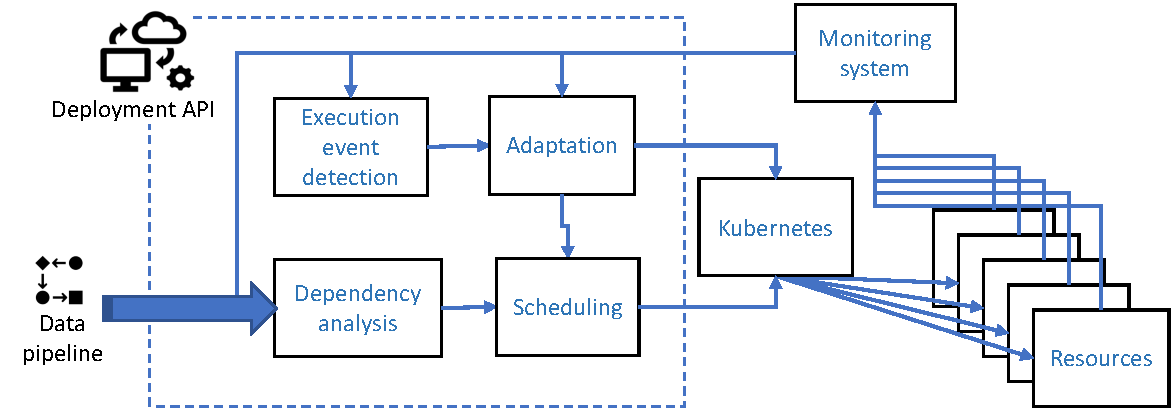
\includegraphics[width=0.8\textwidth]{pdf/data_cloud_arch.pdf}
        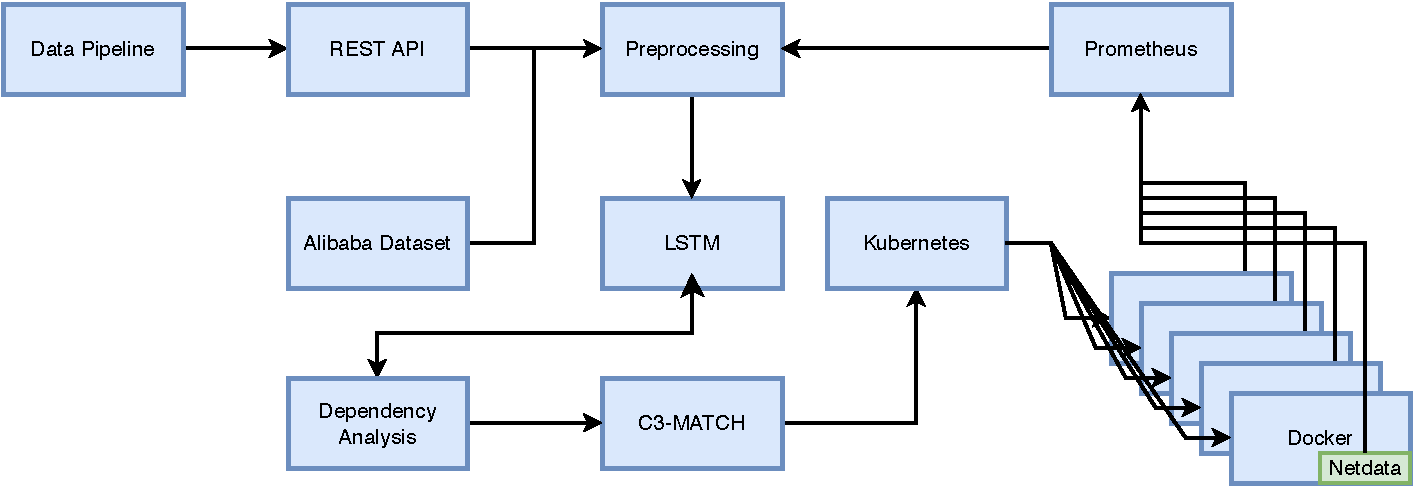
\includegraphics[width=0.99\textwidth]{figures/saa_diagram.pdf}
        \caption{\SAA Architecture}
        \label{fig:data-cloud-architecture}
    \end{figure}

      \paragraph{Data Pipeline} consists of tasks provided by users that are to be deployed on the Computing Continuum. These tasks are forwarded to a REST API on our endpoint.

      \paragraph{REST API} enables the integration of the \SAA{} scheduling and adaptation tool with deployment and orchestration systems.

      \paragraph{Alibaba Dataset} is used to train the prediction model on real data traces consisting of tasks provided as a pipeline to a GPU cluster. The dataset is further described in chapter \nameref{ch:evaluation-and-results}.

      \paragraph{Preprocessing} is used to transform the data coming from either the data pipeline or the Alibaba dataset into a form that is possible to be fed to the machine learning models for training and inference. The methods used for preprocessing are described in section \ref{sec:data-preprocessing-techniques}.

      \paragraph{LSTM} deep neural networks are used to predict the resource utilisation for the tasks incoming from the data pipeline.
      The predicted resources are CPU and memory and both are predicted for each task. 
      Further description of the LSTM variants used is found in section \ref{fig:lstm-model-architecture}.

      \paragraph{Dependency analysis} orders the candidate tasks scheduled on each resource in a preference list based on the aggregate pipeline communication time to each task.
      
      \paragraph{Scheduling with \CMATCH} maps the pipeline tasks to the resources using a matching theory algorithm, applied to the task and resource preference lists in response to infrastructure drifts.
    
    % \paragraph{Adaptation } dynamically applies re-scheduling or migration of the tasks based on the analyzed monitoring received from the execution event detection. Both the scheduling and adaptation interact with the deployment and orchestration system to perform the deployment and adaptation of the tasks.
    
      
      \paragraph{Netdata} is deployed on all computing devices that are used to execute the tasks and receive them from the \CMATCH scheduler. Netdata is a monitoring tool that tracks the status of a resource it it deployed on.
      The capabilities and usage is described in more details in section \ref{sec:netdata-third-party}.

      \paragraph{Prometheus} fetches monitoring data from resources that have Netdata deployed to identify SLO violations or anomalies during execution. Additionally, it is used to aggregate and store monitoring traces of executed tasks to later use them for fine-tuning the LSTM model.
      Further details are found in section \ref{sec:prometheus-third-party}.

      \paragraph{Docker} is used to containerise tools such as Netdata and Prometheus and deploy them on a Kubernetes cluster. Also the tasks in the data pipeline are containerised and deployed on the resources of the Computing Continuum \cite{kimovskiBigDataPipeline2022}.
      Additional details are found in section \ref{sec:docker-third-party}.


    \subsection{Scheduling}
    \label{sec:scheduling-saa-background}

      The scheduler is \emph{capacity-aware algorithm} designed for asynchronous data processing workflows called \CMATCH.

      \begin{quote}
          We model the asynchronous communication between microservices using data element queues, expressing temporary storage of communication data elements \cite{mehranMatchingbasedSchedulingAsynchronous2022}.
      \end{quote} 
      \CMATCH defines a scheduling approach that is similar to a matching game, where both the tasks in the pipeline and the available resources participate in this game.
      On the task side, each task ranks the available resources based on its resource preferences.
      On the resource side, each resource also ranks the deployable tasks based on its task preferences.

    \subsection{Adaptation}
    \label{sec:adaptation-saa-background}

        The adaptation process consists of multiple components that communicate with each other via API.
        The usual execution order is represented by the order in the components mentioned in this section.
        

        \paragraph{Monitoring and Analysis Component}
        \label{par:monitoring-component-saa-background}
        
          is responsible for monitoring the resources and tasks and storing traces of the behaviour of the system on the disk.
          This is necessary to be able to analyse the correlations of the tasks and resources and train the LSTM model to generate accurate predictions for future task deployments. Each available resource will run a \nameref{sec:netdata-third-party} container in the background that monitors its current state of it. 
          This component runs a \nameref{sec:prometheus-third-party} instance that periodically scrapes all resources with a Netdata endpoint and checks each of them for rule violations. Prometheus includes a rule-based approach that triggers events in case a defined rule is broken by a resource.
          In this context, rules denote the expected limits of a resource such as a CPU utilisation that must not exceed a specific percentage value.
          Otherwise, an event is triggered that is sent to the Adaptation component (see \ref{par:adapt-component-saa-background}) that will adapt the affected resource to function in expected limits again.
      
        
        \paragraph{Adaptation Component}
        \label{par:adapt-component-saa-background}
        
          uses a trained LSTM model to adapt the hardware requirements of the current tasks that reside in the task pipeline.
          Tasks are provided with initial hardware utilisation limits that are not to be exceeded. As already stated in \ref{sec:public-cloud-provider-traces-in-available-data-related-work}, the majority of tasks utilise more hardware resources than they require. The Adapt Component analyses the tasks, their properties and their ordering and adapts the hardware utilisation based on the estimations done by the LSTM model.

    \begin{figure}[h!]
        \centering
        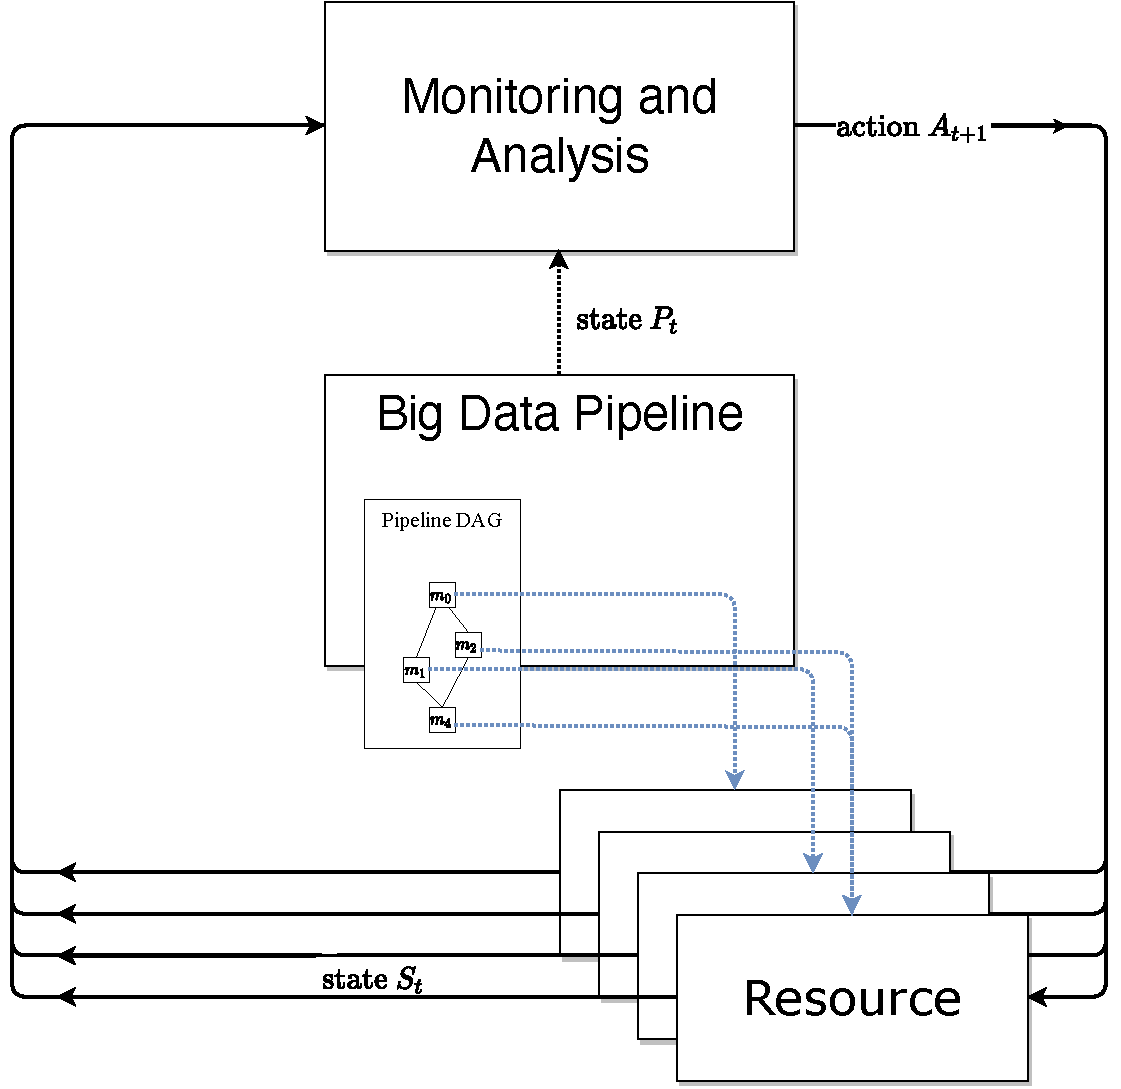
\includegraphics[width=0.95\textwidth]{figures/monitoring_with_inner_resources.drawio.pdf}
        \caption{Adaptation Loop}
        \label{fig:adaptation-loop}
    \end{figure}

    \subsection{The SAA Approach}

      The SAA adaptation approach is defined as a loop, that cyclically updates every component contained in the loop.
      The adaptation loop is shown in figure \ref{fig:adaptation-loop} and consists of the Big Data pipeline and the \emph{resources} containing all registered and monitored to the \emph{Monitoring and Analysis} component. 
      Both the Big Data pipeline and the resources send the gathered monitoring information at a time step $P_t$ or $S_t$ respectively to the \emph{Monitoring and Analysis} component, where $t$ denotes the current time step.

      The Monitoring and Analysis component then uses the monitoring data $P_t$ and $S_t$ and calculates an action $A_{t+1}$ as an update for the resources, where $t+1$ denotes the next time step.
      This received action $A_{t+1}$ is then used by the Resource components to reconfigure the resources if necessary.
      The adaptation uses monitoring of tasks and resources to retrieve the monitoring data $P_t$, $S_t$.
      The monitoring component is necessary to obtain information about failures or performance fluctuations along with under-, and over-utilisation of resources.
      The monitoring data, therefore, provide feedback if a resource can handle the additional load, and thus, more tasks will potentially be mapped to it for execution. 
      In case the resource is not capable of handling the current load, less demanding tasks will be mapped to that resource in future scheduling cycles and it will be reconfigured accordingly.

      A monitored resource information consists of the CPU, memory and storage utilization, in addition to network bandwidth usage.
      The Big Data pipeline and resources send their monitoring data $P_t$, and $S_t$ respectively to the Monitoring and Analysis component.
      Afterwards, given those monitoring data, the analyser will determine the next action $A_{t+1}$ of the resources.
      The monitoring feedback will be periodically retrieved from all registered resources and provided to the analyser.
      In case of a resource side failure, the monitoring mechanism will be alerted of the occurred anomaly.  
      The analyser uses this monitoring data to decide if any actions $a \in A$ on the current scheduling plan have to be applied.
      The following actions $A$ are considered in the adaptation approach:

      \subsubsection*{Resource load within expected parameters $(S_1)$} 

        When tasks on resources are well mapped and no action has to be taken for these resources, this is denoted in the action set $A_{t+1}$ as the state $S_1$. This state is achieved when a resource is running within expected parameters, the estimated time of completing a task is not exceeded or other anomalies occur.

      \subsubsection*{Resource load under expected parameters $(S_2)$}

        When the monitoring component detects under-utilization of a resource, tasks of the pipeline are mapped to it to be efficiently utilized. This state is categorized as $S_2$ in the analyser and the action set will be modified to improve the utilization of resources grouped into $S_2$. 

      \subsubsection*{Resource load over expected parameters $(S_3)$} 

        If a resource is over-utilized, there are multiple options. If it is detected that horizontal scaling solves the over-utilization and the resource instance is capable of being scaled up, it will be reconfigured to be within expected utilization levels. Furthermore, if an ill-defined task is detected and mapped to a resource that isn't capable to fulfil the computation within a reasonable time frame, this task will be migrated to another resource. 
        This is categorized as $S_3$ in the analyser, and the action set will be modified so that resources grouped in $S_3$ will be less utilized with the upcoming updates of the action set \cite{kimovskiBigDataPipeline2022}.


  \section{Third-Party Tools}
  \label{sec:third-party-tools-architecture}

    In this section, the third-party tools that were used in this master's thesis are briefly described and where they were used.
    These tools range from deployment components and machine learning frameworks used to implement and train the machine learning models.

  \subsection{Docker}
  \label{sec:docker-third-party}

    Docker \cite{dockerDockerDocumentationOverview2023} is an open-source platform for automating the deployment of applications inside containers. A container is a standalone executable package that includes everything needed to run a piece of software, including the code, runtime, libraries, environment variables, and system tools.
    Abstracting applications as containers provide a consistent and reproducible environment, which makes it easier to move applications between development, testing and production environments.
    Containers are often used to package an entire application with all its dependencies into a single container image that can easily be moved and run on any device with a Docker runtime.
    The docker toolbox provides tools for building, shipping and running containers, including a runtime environment for containers called Docker Engine, Docker Hub (a repository for storing and sharing images) and the Docker CLI to be able to interact with Docker via a command-line interface.
    In the master's thesis, Docker is used for containerising the monitoring tool mentioned in section \ref{sec:kubernetes-third-party} as well as the LSTM model described in section \ref{sec:lstm-architecture-and-implementation}.
    This is done to easily deploy them inside the distributed system in a scalable manner. 

  \subsection{Kubernetes}
  \label{sec:kubernetes-third-party}
    Kubernetes \cite{the-linux-foundationKubernetesDocumentationGetting} is an open-source platform for automating the deployment, scaling, and management of containerized applications. It was originally developed by Google and is now maintained by the Cloud Native Computing Foundation (CNCF).
    Kubernetes provides a way to manage and organize containers (such as \nameref{sec:docker-third-party} containers) at scale, making it easier to deploy, update, and maintain applications. It does this by abstracting the underlying infrastructure and providing a unified API for managing containers.
    Kubernetes helps to automate many of the manual tasks involved in deploying and managing containers, such as scaling up or down the number of replicas of an application, rolling out updates, and managing network and storage resources. It also provides features for scaling and self-healing, allowing your applications to be more robust and resilient.
    Kubernetes has become a popular platform for deploying cloud-native applications and is widely used by organizations of all sizes across various industries.

    \subsection{NetData}
    \label{sec:netdata-third-party}

      Netdata \cite{netdataGettingStartedLearn2023} is an open-source tool that collects real-time metrics, including CPU usage, disk activity, bandwidth usage and furthermore.
      The reason we chose Netdata for monitoring is that it is a lightweight tool mostly written in C, Python and Javascript and it requires minimal resources, which is necessary when monitoring edge devices.
      One of its major features is that it runs without interrupting any of the applications running on the same device. This is achieved by only using idle CPU cycles while running.
      Netdata provides an in-browser dashboard to analyse each metric in real time with help of visual representation. As an example, a screenshot was taken of a cloud resource in our system as can be seen in \ref{fig:netdata-dashboard}.
      \begin{figure}[h!]
          \centering
          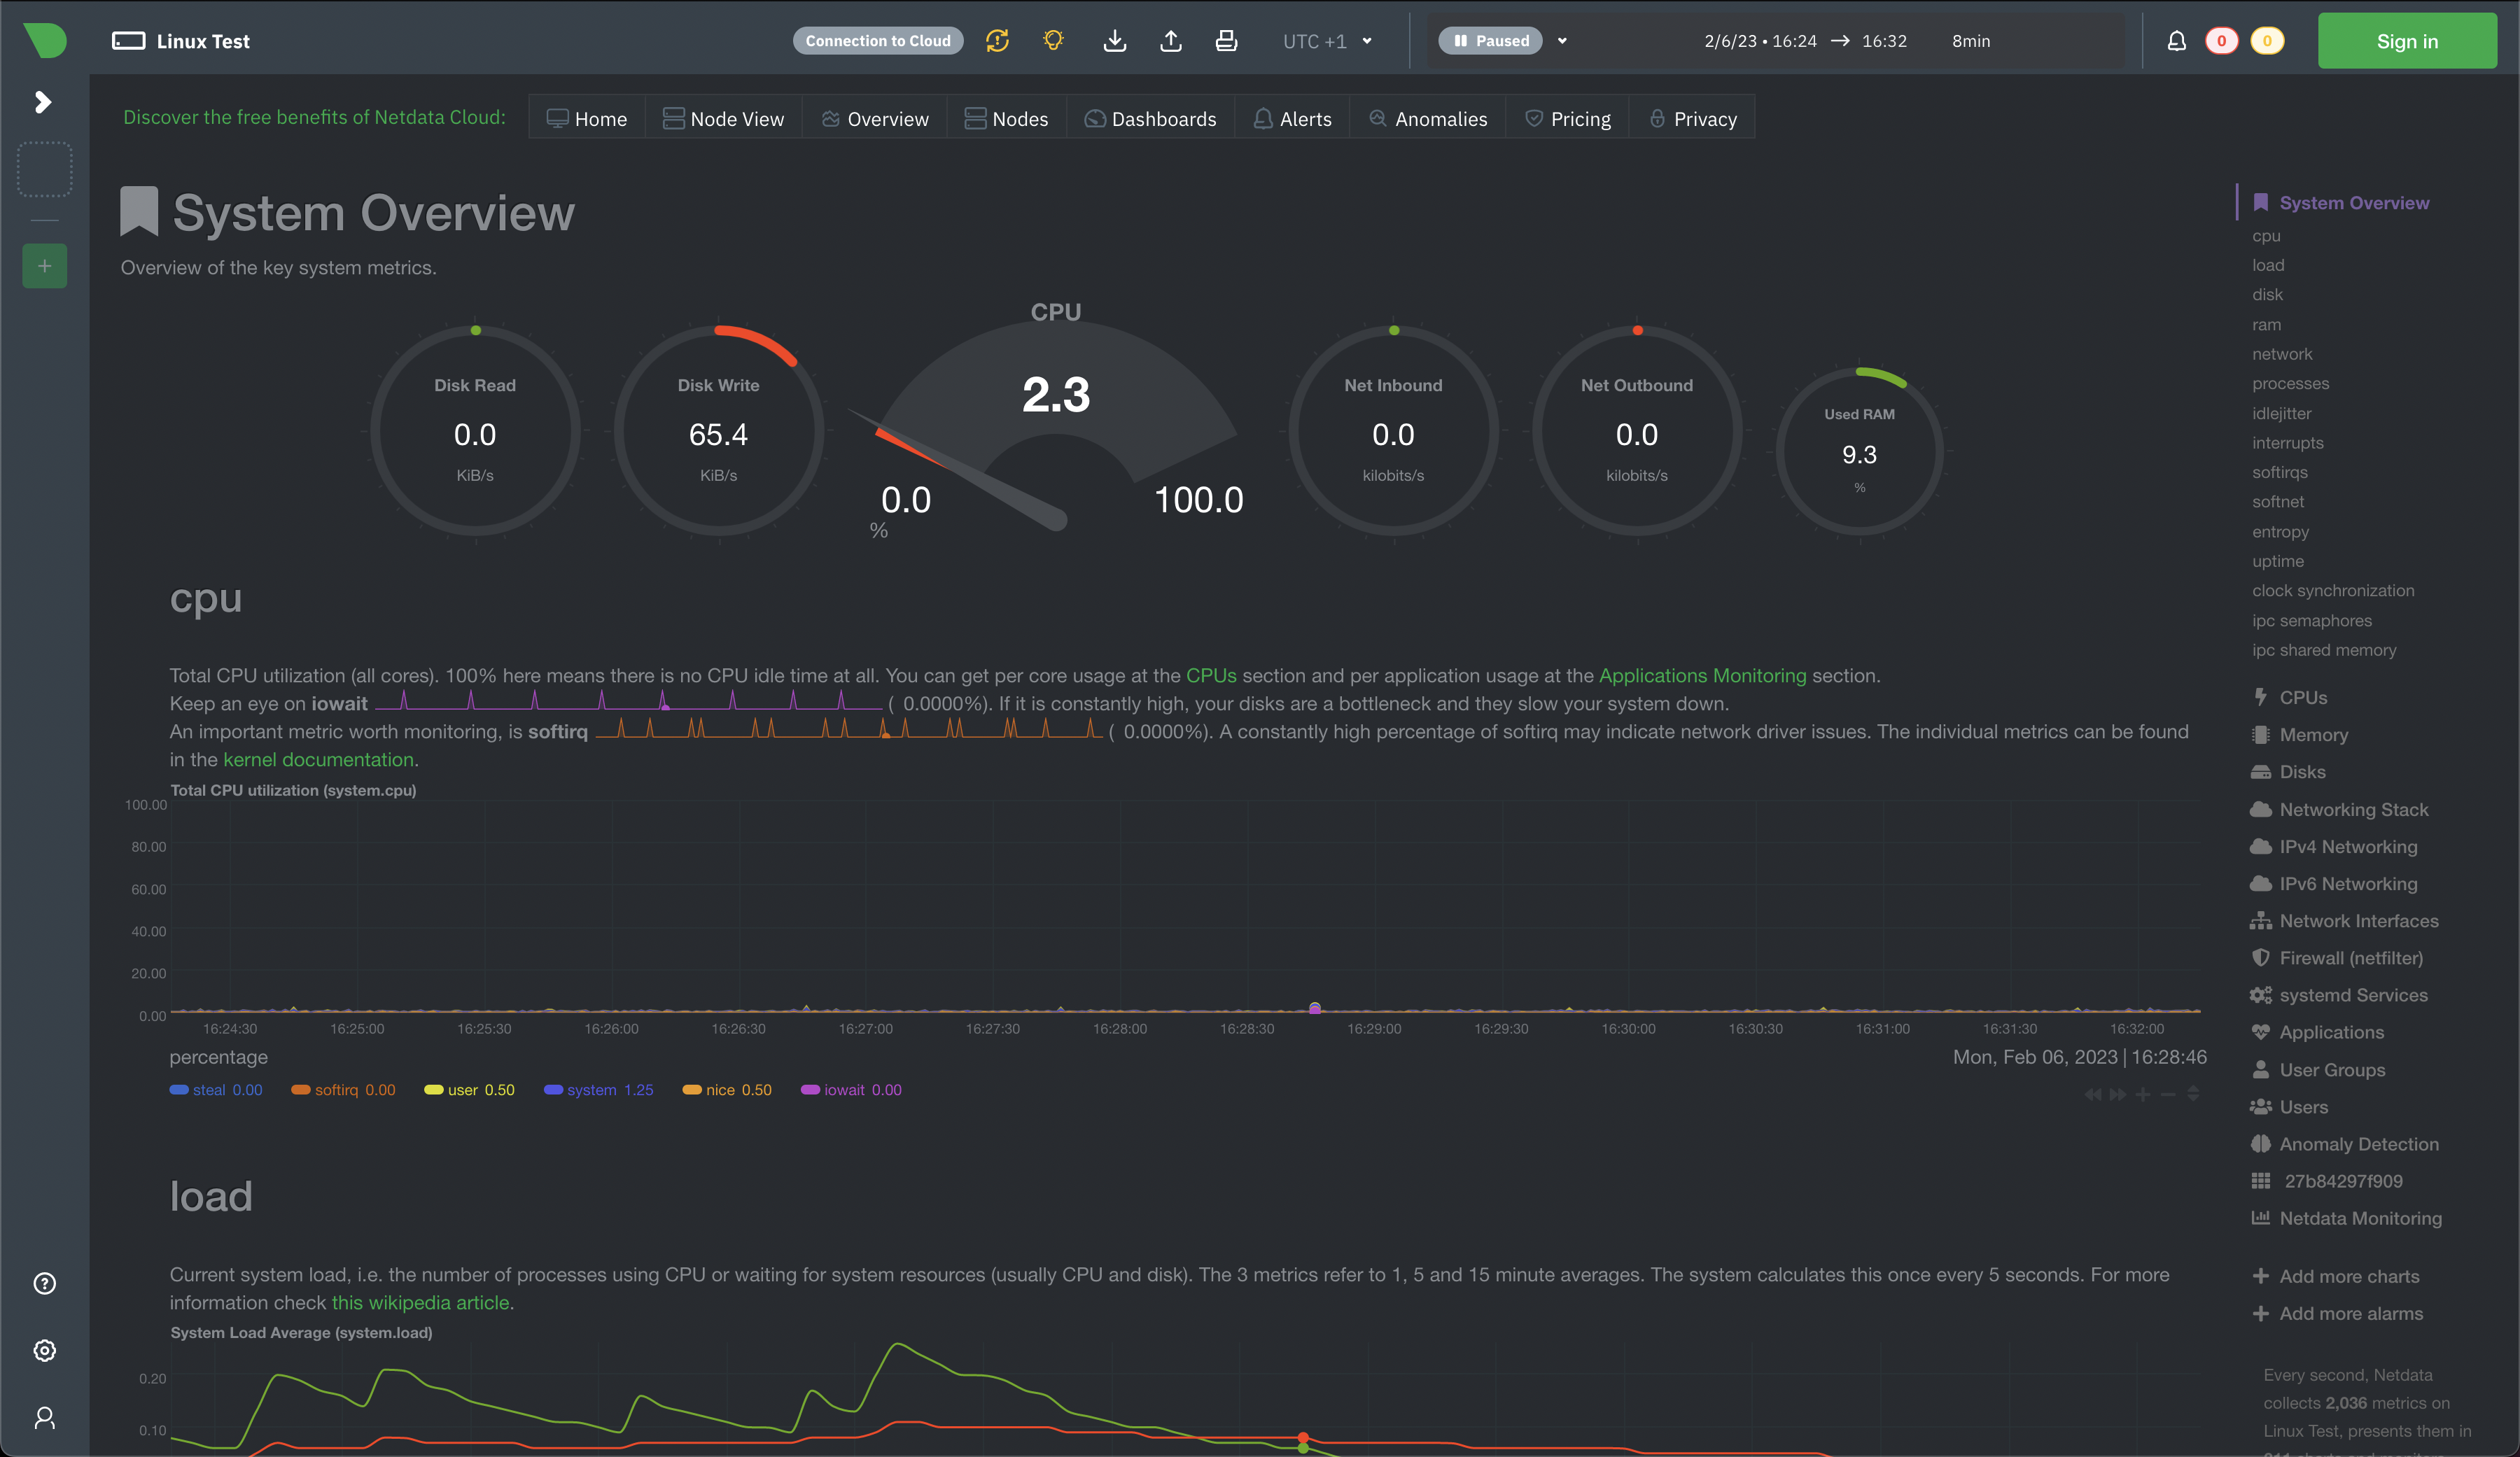
\includegraphics[width=0.95\textwidth]{figures/netdata.png}
          \caption{Netdata Dashboard Example}
          \label{fig:netdata-dashboard}
      \end{figure}
      Netdata has a vast amount of support for other tools to gather data. 
      One of the supported tools is \nameref{sec:prometheus-third-party}, which is used to scrape the monitored data from all resources that have Netdata installed. 

    \subsection{Prometheus}
    \label{sec:prometheus-third-party}
    
      Prometheus \cite{prometheusOverviewPrometheus} is an open-source application used for monitoring and alerting of events and is designed to run across various platforms in a scalable and easily deployable manner.
      Same as Netdata it records in real-time, and stores the gathered metrics in a time series database by using an \emph{HTTP pull model}. It also allows real-time alerting via a rule-defining configuration and also has a flexible query language called \emph{PromQL}, that enables the retrieval and processing of the gathered data. Prometheus has great integration with other tools such as Netdata.
      In the project, it is used inside a monitoring master node that is continuously scraping all resources that have Netdata installed for monitoring data. In case a predefined rule is broken at a monitored resource, such as CPU over-allocation, Prometheus triggers an event that notifies the Adaptation Component (see section \ref{sec:scheduling-and-adaptation-approach-architecture}) to be able to take measurements.


    \subsection{Pandas}
    \label{sec:pandas-third-party}

      Pandas \cite{pandasPandasDocumentationPandas} is an open-source library created for Python and its main purpose is to provide tools for data analysis and manipulation as well as data structures for large-scale numerical tables and time series data.
      Pandas allow importing data from various file formats such as \emph{comma-separated values (CSVs)}, which is the file format that Alibaba chose to store the monitoring traces.
      These CSV files are imported into \emph{Pandas DataFrames}, which is the main data structure used for data manipulation with Pandas. DataFrames are used to merge the different datasets to create the training and test datasets for the LSTM model, and additionally, most of the data analysis is also done with the help of the functions that are built into the DataFrame class.

    \subsection{PyTorch}
    \label{sec:pytorch-third-party}
      PyTorch \cite{the-linux-foundationPyTorch} is an open-source machine learning library for Python, developed by Facebook's AI Research lab (FAIR) but is now part of the \emph{Linux Foundation umbrella}. It provides tensor computation (similar to NumPy) with strong support for deep neural networks built on a tape-based autograd system. PyTorch is designed to provide flexibility and ease of use, with a focus on deep learning and neural networks. It can be used for various tasks such as natural language processing, computer vision, and speech recognition.
      PyTorch also supports deployment on various platforms, including CPUs, GPUs, and TPUs, and has an active community of users and contributors that continue to improve and expand its capabilities.
      PyTorch is used to build the LSTM model (see section \ref{sec:lstm-architecture-and-implementation}) and the loss function (see section \ref{sec:penalty-mse-loss-function-architecture-and-implementation}) to train the models and use the trained variants for inference of resource utilisation.


  \section{Data Preprocessing}
  \label{sec:feature-engineering-data-preprocessing-architecture}

    Data preprocessing (also referred to as feature engineering) is the process of designing artificial features, that is, to model features that are used as the inputs for a machine learning (ML) model either during training or inference to make predictions. In short, it is the development of new data features from raw data.
    It is a very important step in machine learning since the later prediction performance depends on the quality of the data.
    The accuracy of an ML model heavily relies on a well-composed and precise set of features to make reliable predictions. Regardless of the data or ML architecture, if a feature set is not well-suited, it does have a direct impact on the ML model.
    \begin{quote}
      Feature engineering is a machine learning technique that leverages data to create new variables that aren't in the training set \cite{patelWhatFeatureEngineering2021}.
    \end{quote}
    Feature engineering involves the extraction and transformation of variables of a raw data source. This process is necessary to be able to use the data for the training of an ML model and successfully use its inference to make predictions.
    The steps required in feature engineering include \nameref{sec:feature-extraction-preprocessing-architecture} and \nameref{sec:feature-cleansing-preprocessing-architecture} followed by feature creation and analysis (see section \ref{sec:feature-creation-analysis-preprocessing-architecture}).
    It can produce new features to enhance the model accuracy and simplify and speed up data transformation.

    \subsection{Feature Extraction}
    \label{sec:feature-extraction-preprocessing-architecture}

      Feature extraction is the process of collecting and assembling all the data that is required for the ML training into a feature set.
      Data often resides in multiple data sources, therefore collecting training data is a challenging process since those different data sources need to be connected for it to be usable. Furthermore, data sources often have vastly different formats and types, which also needs to be taken into account. 
      Feature extraction also faces the challenge of not distorting the original relationships or significant information of the raw data and also compressing the amount of data into manageable quantities for the ML models to process and train on.
      The Alibaba cluster traces consist of a multitude of datasets, each with its respective focus. Because of the distributed nature of the data, first, the common key features were required to be analysed to be able to later join the data based on these common key features to an actual training and test dataset.

    \subsection{Feature Cleansing}
    \label{sec:feature-cleansing-preprocessing-architecture}

      Feature cleansing is the process of cleaning a dataset. 
      A major part is to add missing values or to remove data points that are not beneficial for the training of an ML model. 
      In the Alibaba dataset, all tasks were removed that did not successfully finish their execution. The reason why the cluster of failed tasks was excluded from the training was that the ML model should be trained on successfully finished tasks since it was not stated what the reason for the failure of the tasks was and adding failed tasks could, in this case, lead to unwanted behaviour when predicting incoming tasks. And therefore, it was deemed a better approach to not include those tasks. 
      This process is shown in listing \ref{lst:drop-failed-tasks}, where only tasks will be kept that had their feature column set to \texttt{'terminated'}, which states that they did successfully terminate their execution.
      \lstinputlisting[
        language=Python, 
        caption=Dropping Failed Tasks from DataFrame, 
        label={lst:drop-failed-tasks},
        style=codestyle
        ]{code_samples/drop_failed_tasks.py}
      After dropping all failed tasks, the feature column \texttt{status} is dropped from the dataset since it now does not provide any information.
      Next, other feature columns are dropped as well that are either not necessary for the training or inference of the ML model or are duplicated columns that were added by the Pandas framework after joining the DataFrames. Dropped columns contain fields such as \emph{read, write, instance name, instance ID, worker-pool name, group, user and status\_t}, where status\_t is simply a duplicated column that was appended while doing a join operation. Feature cleansing also involves the task of ensuring that the correct data types are used for each dataset. In the case of the mentioned dataset, it was necessary to denote the feature field \texttt{start\_date} as a time-stamp as well as the index for the dataset, to ensure a time-series-based ordering of the data. Also, fields such as the \emph{number of instances} were declared as floating point numbers. To ensure that this will not result in unwanted behaviour, this field data type was changed to an unsigned integer.

    \subsection{Feature Creation and Analysis}
    \label{sec:feature-creation-analysis-preprocessing-architecture}

      Feature creation involves the process of data labelling.
      Data labelling identifies data such as images, and text files and adds meaningful and informative labels to it by creating new variables which will be the most helpful to the ML model. This is done to provide the data labels as context to the ML model so it can learn from it. Data labelling is required for various use cases in \nameref{sec:supervised-learning} since ML models of that category require labels to train on. Features that were created for the datasets that later are fed into the LSTM model are one-hot encoded feature columns. These were either generated from the task type, which is used to differentiate between the various tasks and is used to enable the model to comprehend categorical data for training and inference. Similarly, the \emph{number of instances} is one-hot encoded to provide additional information about a task by providing categorical data as encoded feature columns. The one-hot encoding method and how it is applied is described in more detail in section \nameref{sec:one-hot-encoding-preprocessing-architecture}.

    \subsection{Feature Analysis}
    \label{sec:feature-analysis-preprocessing-architecture}
    
      Feature analysis often uses visualisation like histograms, scatter, box and line plots to analyse if the created feature data set is correct. Feature analysis is also used to discover patterns, spot anomalies, check assumptions or test a hypothesis.
      The analysis of features and results is done in chapter \nameref{ch:evaluation-and-results}.

    \subsection{Feature Selection}
    \label{sec:feature-selection-data-preprocessing-architecture}

      Feature selection is the process of reducing the number of input variables of a feature set when developing a predictive model.
      Feature selection is simply the process of selecting and excluding given features without changing them as is done with \emph{dimensionality reduction}.
      A reduction of the number of input variables is desirable to both reduce the computational cost of training a model and in some cases, it also increases the prediction performance of the model.

        % mention the iterations and the inclusion of more features

  \section{Data Preprocessing Techniques}
  \label{sec:data-preprocessing-techniques}

    In this section, the data preprocessing techniques that are used on the datasets used in this thesis are further elaborated.

    \subsection{One-hot Encoding}
    \label{sec:one-hot-encoding-preprocessing-architecture}

    One-hot encoding \cite{fawcettDataScienceMinutes} is used to represent categorical data of a finite set by an index in that set, where only one element has its index set to $1$, and all other values are assigned the value $0$.
    This technique is useful when categorical data should be fed to a machine learning model since many model architectures can only handle numerical values, making it necessary to transform strings or other data types to numbers.
    \begin{quote}
      One hot encoding is a process of converting categorical data variables so they can be provided to machine learning algorithms to improve predictions. \emph{One hot encoding is a crucial part of feature engineering for machine learning} \cite{fawcettDataScienceMinutes}.
    \end{quote}
    The one-hot encoding technique is used for the categorical data of \emph{task type}, where each type of task is represented as an index in the task-type vector. Similarly, one-hot encoding is used to classify a different number of instances (or Kubernetes Replicas) into clusters, that are then mapped to an index of the encoded feature vector.
    
    To generate one-hot encoded feature vector columns in the application, we used the Python framework \texttt{Pandas}.
    Pandas is a popular framework that was designed to handle big datasets that are represented with their internal \texttt{Series} and \texttt{DataFrame} data types, where \texttt{Series} is a feature column and a DataFrame is a collection of Series or a feature vector. The process of generating one-hot encoded columns for a DataFrame is shown in the listing \ref{lst:one-hot-encoding}.
    To generate one-hot encoded columns for a DataFrame, the column or row with the categorical data has to be isolated.
    In line 2, the \texttt{instances} Series is used to generate a new Series that contains the index position for the one-hot encoded feature vector.
    Next, in line 3 the \texttt{get\_dummies()} function of Pandas is used to generate the one-hot encoded feature vector of a DataFrame data type that is stored in a variable called \texttt{dummies}.
    In lines 4-8, the columns of the \texttt{dummies} DataFrame are renamed to be concise with the defined instance clusters. The \texttt{inplace=True} flag is necessary since Pandas usually does not modify DataFrames directly but an operation commonly returns a copy of the modified DataFrame, and this flag omits the copy process and renames the columns directly in the DataFrame.
    \lstinputlisting[
      language=Python, 
      caption=One-Hot Encoding Pandas Example, 
      label={lst:one-hot-encoding},
      style=codestyle
      ]{code_samples/one_hot.py}
      
    Finally, the one-hot encoded feature vector \texttt{dummies} is joined with the training DataFrame called \texttt{training\_df} and the result is stored in the variable \texttt{inst\_df}. An example one-hot encoding of the first few values of the training DataFrame is shown in table \ref{tab:one-hot-encoding-instances}, where $task_0$ is categorised to be part of instance cluster $0$ and the following two tasks $task_1, task_2$ are part of instance cluster $3$.
    \begin{table}
      \centering
      \caption{Example of One-Hot Encoding the Instances}
      \begin{tabular}{|l|rrrr|}
        \toprule
        index &  inst\_clust\_0 &  inst\_clust\_1 &  inst\_clust\_2 &  inst\_clust\_3 \\
        \midrule
        0 &             1 &             0 &             0 &             0 \\
        1 &             0 &             0 &             0 &             1 \\
        2 &             0 &             0 &             0 &             1 \\
        \bottomrule
      \end{tabular}
      \label{tab:one-hot-encoding-instances}
    \end{table}

    Using one-hot encoding enables the LSTM model to additionally learn from categorical features such as the type of task (see evaluation scenario \nameref{sec:adding-task-knowledge-evaluation-scenarios}) and also to learn and infer from the number of instances (or \nameref{sec:kubernetes-third-party} replicas). 
    These further details about each task enable the ML model to better and more accurately react to the given sequence of tasks.

    \subsection{$z$-Score Normalisation}
    \label{sec:data-standardisation-data-preprocessing-architecture}
      % https://towardsdatascience.com/what-is-feature-engineering-importance-tools-and-techniques-for-machine-learning-2080b0269f10
      $z$-Score Normalisation (also referred to as \emph{standardisation}) is a process of scaling values of a dataset by first calculating its standard deviation and accounting for it. In case the standard deviation of features is different, then the range of those features will likewise differ. As a result, the outliers in the characteristics are reduced.
      In order to calculate a distribution of the data with a mean of $0$ and a variance of $1$, all the data points are first subtracted by their mean and the result of that is then divided by the variance of the distribution.

      \begin{pabox}{Mean}
        \label{def:mean}
        The mean $\mu$ is calculated with the formula:
        $$\mu = \frac{1}{N}\sum_{i = 1}^{N}\left(x_i\right)$$
        where $N$ denotes the number of elements in the dataset and $x_i$ the $i$-th element in that dataset.
      \end{pabox}

      \begin{pabox}{Standard Deviation}
      \label{def:standard-deviation}
        The standard deviation is calculated with:
        $$\sigma = \sqrt{\frac{1}{N} \sum_{i = 1}^{N}\left(x_i - \mu\right)^2}$$
      \end{pabox}

      \begin{pabox}{$z$-Score Normalisation}
      \label{def:standardisation}
        The standardisation is calculated by the formula $$Z = \frac{x - \mu}{\sigma}$$
      \end{pabox}

      The $z$-score normalisation of data points is used to preprocess the feature dataset that is fed to the LSTM model while training or inferring tasks. Standardising the feature dataset is preferred to normalisation (see section \ref{sec:data-normalisation-data-preprocessing-architecture}) since the impact of outliers is reduced compared to the normalisation scaling method.

    \subsection{Normalisation}
    \label{sec:data-normalisation-data-preprocessing-architecture}

      In \textbf{normalisation}, all values in a data set are scaled in a specified range between $0$ and $1$ via normalisation and represented as floating-point numbers.
      The normalisation of data does not influence the distribution of the features, but it does increase the effects of outliers due to the lower standard deviation after the modification. Because of this, it is necessary to deal with outliers before applying normalisation to a data set.
      
      \begin{pabox}{Normalisation}
        \label{def:normalisation}
        The normalisation scaling formula and its parameters are defined as follows:

        The minimum value of a dataset is denoted as $x_{min}$ and the maximum value as $x_{max}$.
        The value $x$ denotes a data point that will be scaled between $0$ and $1$ and its new value is denoted as $x_{new}$.
        $$x_{new} = \frac{x - x_{min}}{x_{max} - x_{min}}$$

        
      \end{pabox}
      The normalisation of data points is used for the label dataset that contains the labels that the ML model should predict (i.e. the hardware utilisation of resources). The normalisation is used for the label dataset because its values of it are transformed to a standard scale without distorting the difference between the values. This behaviour is useful when predicting the actual values in the label dataset.

      \begin{pabox}{De-Normalisation}
        The de-normalisation is used to rescale the estimation done by the LSTM model into the range of the actual values. The formula for calculating the inverse of the normalisation is:

        $$x = x_{new} * (x_{max} - x_{min}) + x_{min}$$
        The old value $x$ is calculated by simply rearranging the normalisation formula and de-normalising the normalised value $x_{new}$.
      \end{pabox}
      The de-normalisation is used to rescale the predicted values forwarded by the LSTM model to the actual data range.
      This is required since the LSTM model is trained to predict normalised values since this commonly results in more accurate predictions.
    
  \section{LSTM Architecture}
  \label{sec:lstm-architecture-and-implementation}

    In this section, the architecture of the LSTM model is elaborated.
    This involves the description of the different layers that are used as well as some operations that are required to improve the prediction of the model.
    The LSTM model was implemented with \nameref{sec:pytorch-third-party}, an open-source machine-learning library for Python. 
    \begin{figure}
      \centering
      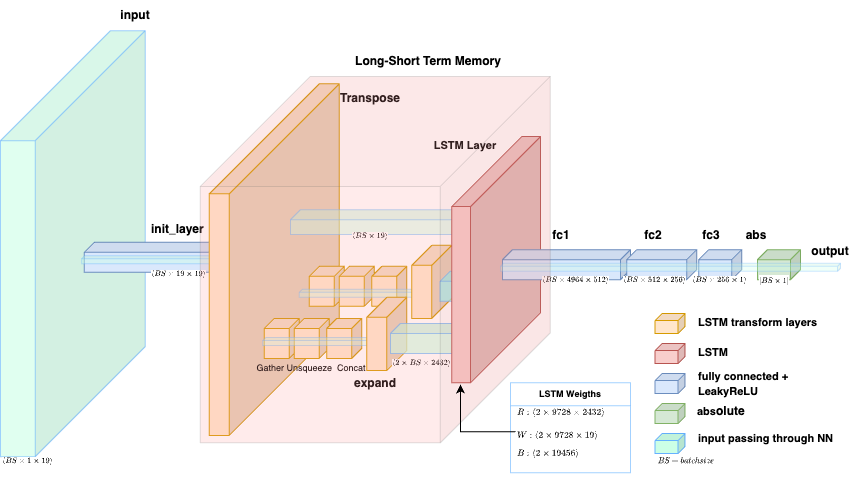
\includegraphics[scale=0.45]{figures/current_lstm_model.png}
      \caption{LSTM Model Architecture}
      \label{fig:lstm-model-architecture}
    \end{figure}

    The LSTM model implementation is called \texttt{UtilizationLSTM} and is of type \texttt{Module}. This is a default parent class for neural networks that are implemented in PyTorch.
    The class constructor \texttt{\_\_init\_\_()} has four parameters. First, is the instance reference \texttt{self} that is used to access functions and variables of an instance. 
    The available instance variables are \emph{input size, hidden size, number of layers} and \emph{device} that holds the reference to the hardware that will compute the training of the neural network.
    PyTorch enables the training of neural networks on graphical computing units (GPU) which accelerates the training process. For being able to train on a GPU, the NVIDIA API CUDA (Compute Unified Device Architecture) needs to be installed on the device, in order to send the LSTM model on the GPU and train it on incoming data batches. 
    Next, is the input size that refers to the number of feature set columns that were selected by the \nameref{sec:feature-selection-data-preprocessing-architecture} process.
    The hidden size value in the parameters also refers to the hidden layer size of the LSTM model that is used to variate the size of the model and its capabilities to remember long-term patterns in time series data.
    Finally, the number of layers refers to how many \nameref{sec:stacked-lstm} layers should be applied.
    For the \nameref{sec:evaluation-scenarios}, a default of two stacked layers is used. When using two stacked LSTM layers, the size of the hidden layers of the model is doubled. This also includes the model output, where both hidden state outputs are returned by the \texttt{forward} function.
    The reason why an estimation that is then fed back to the model is returned is to be able to analyse the hidden states of the intermediate model layers.
    \lstinputlisting[
      language=Python, 
      caption=LSTM Constructor, 
      label={lst:lstm-init-function},
      style=codestyle
      ]{code_samples/lstm_init.py}
    Next, the two LSTM models are instantiated in lines 17 and 25 with the parameters from above. One for the prediction of CPU and one for the prediction of memory utilisation. The \texttt{batch\_first} parameter provided to both models defines how the model shall return its estimation, in this implementation, the batch will be returned first, followed by the hidden state and then the internal state.
    
    Then, a sequential layer for both LSTM models is generated by the function shown in \ref{lst:lstm-init-sequential-layer-batchnorm}. This sequential layer consists of three components. Each component is built with the following components:
    
    \begin{pabox}{Rectified Linear Unit (ReLU)}
    \label{def:relu-definition}
      \textbf{Rectified Linear Unit (ReLU)} is a popular function for transforming the summed weighted input from a layer into the activation of a node or output for that input.
      The ReLU function can be mathematically described as $$g(z) = \max \left\{0, z\right\}.$$

    \end{pabox}
    The advantages of ReLU are its computational simplicity, the representational sparsity (being able to output true zero values opposed to $\tanh$ and $sigmoid$), the linear behaviour and the training of deep neural networks via backpropagation was heavily improved when using ReLU compared to more complex methods. The function is linear for values greater than zero which results in ReLU having many of the advantages of a linear activation function when using backpropagation. Yet, ReLU is a nonlinear function since negative values are always output as zero.

    \begin{pabox}{Batch Normalisation}
    \label{def:batch-normalisation-definition}
      \textbf{Batch normalisation (batch norm)} is a generalisation method used to increase the stability and reduce the training time of a neural network layer by re-centring and re-scaling the inputs of the layer.
      Batch normalisation standardises the inputs to a layer for each mini-batch, and the resulting increase in stability reduces the number of required training epochs to train deep neural networks.

      \begin{quote}
        % https://machinelearningmastery.com/batch-normalization-for-training-of-deep-neural-networks/
        Batch normalization provides an elegant way of \emph{reparametrizing} almost any deep network. 
        The reparametrization significantly reduces the problem of coordinating updates across many layers \cite{goodfellowDeepLearning2016}.
      \end{quote}
      Assumptions that a subsequent layer makes during the weight update that regards the spread and distribution of inputs, will not change by a lot of the activations of the prior layer are standardised. 
    \end{pabox}
    \raggedbottom
    Normalising the input batch also has a regularising effect, which leads to a reduction of generalisation errors, similar to the usage of activation regularisation.
    Batch normalisation was proposed to mitigate internal covariate shift. This internal covariate shift occurs because inputs that are forwarded to the neural network and also from each layer have a corresponding distribution that affects the training process because of the randomness of the parameter initialisation and input data.
    Because of the resulting internal covariate shift, the succeeding network layers need to readjust their weights in order to update their state from the data that was forwarded from the proceeding layer with a bias in terms of the distribution of activated nodes. This requirement to readjust to new distributions is even more severe in deep neural networks that have many layers and the increased number of layers amplifies this effect. Batch normalisation reduces unwanted shifts propagated by layers, speeds up the training, and also produces more reliable and general models.
    


    \begin{pabox}{Linear (Fully-Connected) Layer}
      \label{def:linear-layer-definition}
      Linear layers, also known as fully-connected layers connect every input neuron to every output neuron and are commonly used in neural networks. The structure of a neural network consisting of fully-connected layers can be seen in the figure below, where each node is connected to all nodes of the previous and the succeeding layer.
      A linear layer is defined by three parameters, the number of inputs, the number of outputs and the batch size.
      Operations such as forward propagation, activation gradient computation, and weight gradient computations are directly expressed as matrix multiplications.
      \begin{minipage}[t]{1\linewidth}
        \centering
        \vspace*{0pt}
            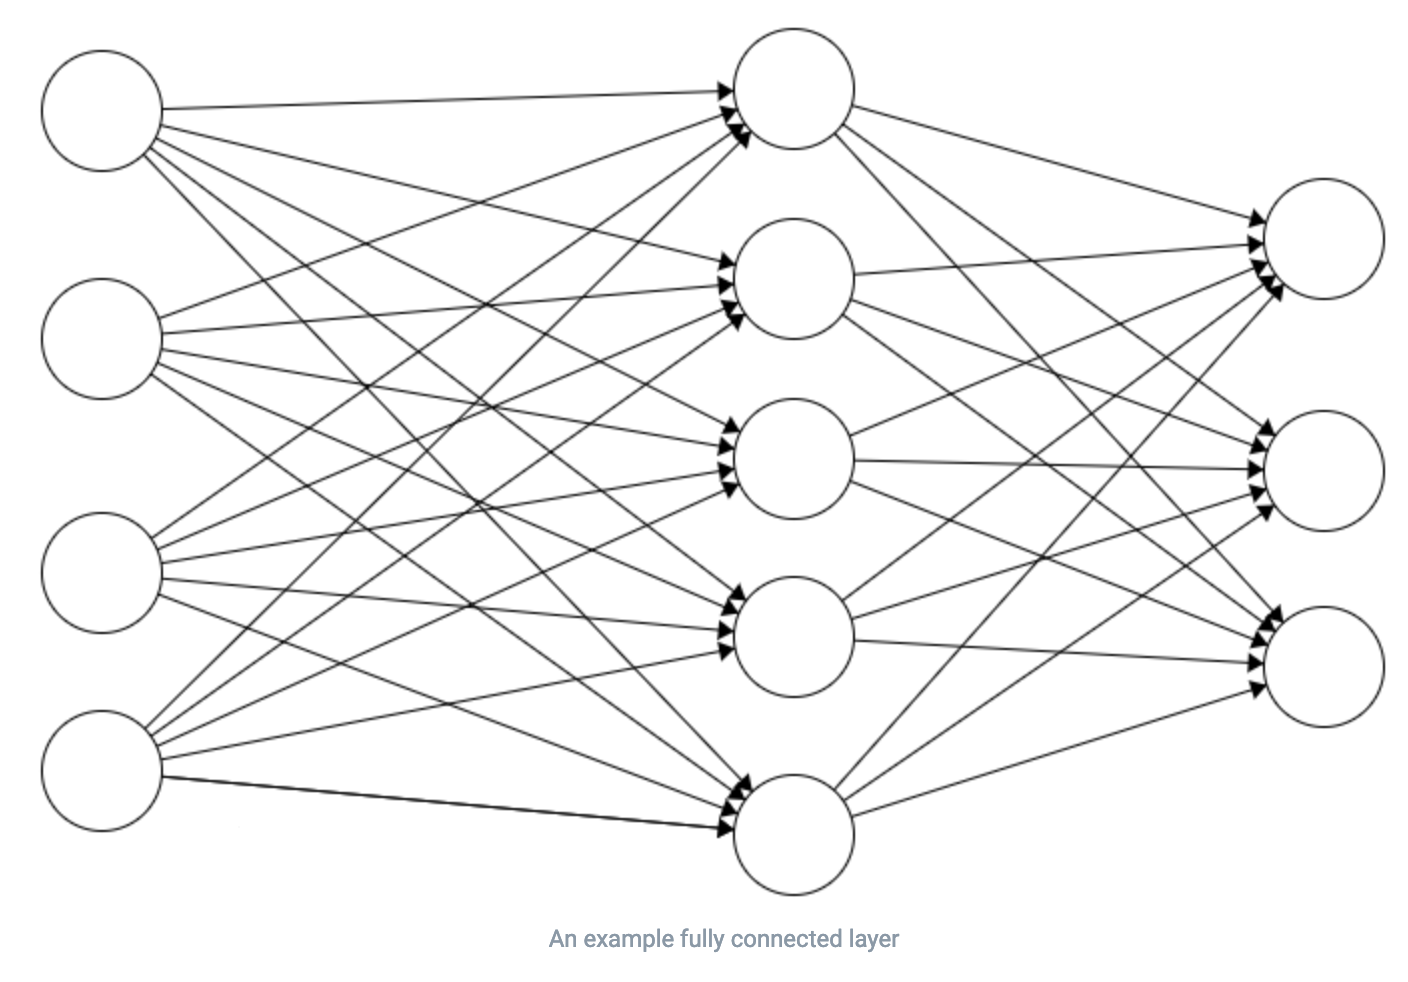
\includegraphics[height=0.25\textheight,width=0.5\linewidth]{figures/fc_layer.png}
            \captionof{figure}{Fully-Connected Layers \cite{FullyConnectedLayer}}
            \label{fig:fully-connected-layers-architecture}
        \end{minipage}

    \end{pabox}
    These LSTM and sequential layers are the core of the machine learning architecture inside the \texttt{UtilizationLSTM} class and are responsible for the estimation of the CPU and memory utilisation and are used by forwarding inputs through each layer until the estimation is calculated.
    The received input is sent to the \texttt{forward} function of the class that expects a PyTorch tensor as the input type.
    
    \lstinputlisting[
      language=Python, 
      caption=LSTM Initialise Sequential Layers with BatchNorm, 
      label={lst:lstm-init-sequential-layer-batchnorm},
      style=codestyle
      ]{code_samples/lstm_init_seq_layer_bn.py}


    As can be seen in figure \ref{fig:lstm-model-architecture} the input vector consisting of a pipeline task batch is forwarded to the \emph{initial lstm layers}. This step is implemented in the LSTM \texttt{forward} function (see \ref{lst:lstm-forward-function}) in lines 8 and 9. The \texttt{get\_hidden\_internal\_state} (see \ref{lst:lstm-init-internal-hidden-state}) function seen on the right side of lines 8 and 9 is used to create the initial internal and hidden state based on the time series batch provided as the \texttt{input} for the model. The input vector is a PyTorch tensor that is then sent to a function that generates the initial hidden and internal state based on the shape of the input vector.
    The general LSTM prediction model is split into two smaller LSTM components that each predict the utilisation of one resource unit. A resource unit is either the CPU usage or the allocated memory. At creation these LSTM components use the length of the input as the expected input size and the quality of the prediction performance heavily depends on the chosen hidden layer size as well as the number of \nameref{sec:stacked-lstm} layers.
    The final LSTM output of either resource unit is then sent to traditional sequential layers that use batch normalisation as the generalisation strategy.
    
    Afterwards, the output of those sequential layers is concatenated column-wise as a label vector of the form $\left[(cpu_1, mem_1), \dots, (cpu_{bs}, mem_{bs})\right]$ where $bs$ denotes the batch size or the number of data points in the batch.
    At line 22 the calculated output is then sliced in order to only include the same amount of elements as the elements of the input vector. This has to be done since using multiple LSTM layers also increases the number of output elements by the simple formula $elements_{input} \times \#layers$. For the estimation of the resource utilisation, only the last estimation section of the output is required since this is the section that contains the prediction of the last LSTM layer.
    In line 25 the absolute values of the output are calculated. This is done to ensure that negative values are not included in the prediction since the hardware utilisation can't be less than zero.

    \lstinputlisting[
      language=Python, 
      caption=LSTM Forward Function, 
      label={lst:lstm-forward-function},
      style=codestyle
      ]{code_samples/lstm_forward.py}

    \lstinputlisting[
      language=Python, 
      caption=LSTM Initialise Internal and Hidden State, 
      label={lst:lstm-init-internal-hidden-state},
      style=codestyle
      ]{code_samples/lstm_get_hidden_int_state.py}


  \section{DataFrame Scaler}
  \label{sec:dataframe-scaler-architecture-and-implementation}

    The \texttt{DataFrameScaler} is a custom class that handles the scaling of datasets that are in the form of a \emph{Pandas DataFrame} data type. 
    The reason for implementing a custom class for this thesis instead of the popular approach of the \texttt{StandardScaler} and \texttt{MinMaxScaler} classes provided by \emph{scikit-learn} is that these third-party classes destroy valuable information about the dataset while scaling it to either be standardised (see \nameref{sec:data-standardisation-data-preprocessing-architecture}) or normalised (see \nameref{sec:data-normalisation-data-preprocessing-architecture}). 
    Information that is not kept when scaling the DataFrames is data point timestamps, which are converted to ascending integer values. Similarly, the column description is also not kept after the scaling, so it is necessary to dynamically create a map of an integer to the column description.
    Because of behaviour, a custom Python class was implemented that scales the DataFrame to a standardised or normalised DataFrame or if required to be fed to the LSTM model converted to a PyTorch Tensor.
    This class ensures that the timestamps of each data point are kept and fed to the LSTM model and also keeps the column descriptions. Additionally, it is possible to define columns that should be ignored while scaling the DataFrame. This is useful for columns that were one-hot encoded (see \nameref{sec:one-hot-encoding-preprocessing-architecture}, \nameref{sec:adding-task-knowledge-evaluation-scenarios}, \nameref{sec:adding-instance-knowledge-evaluation-scenarios}) before the scaling process.
    The \emph{DataFrameScaler} class contains both the logic for standardising and normalising a DataFrame.

    \lstinputlisting[
      language=Python, 
      caption=DataFrameScaler Constructor and Instance Variables, 
      label={lst:dataframe-scaler-init},
      style=codestyle
      ]{code_samples/dataframe_scaler_init.py}

    As shown in lines 2-5 listing \ref{lst:dataframe-scaler-init} the class contains different instance variables to hold the necessary information about a DataFrame, such as the data types of each column.
    The variables in lines 3-5 hold the standard deviation, normalisation DataFrames and the list of the columns that are to be scaled, respectively. The DataFrame values for the standard deviation and normalisation are calculated in the \texttt{fit()} method (see listing \ref{lst:dataframe-scaler-fit}) that resides inside the class.
    These DataFrames are necessary to later be able to scale other data points that share the same distribution as the DataFrame that was used to fit the scaler. 
    This is used for estimations forwarded by the LSTM model that are within the range of normalised values.
    In order to rescale the estimation into the actual range, the \texttt{norm\_dev\_df} is used to transform the data by using the formula for de-normalisation (see \nameref{def:normalisation}).

    \lstinputlisting[
      language=Python, 
      caption=DataFrameScaler Fit Method, 
      label={lst:dataframe-scaler-fit},
      style=codestyle
      ]{code_samples/dataframe_scaler_fit.py}
    The \texttt{fit()} method of listing \ref{lst:dataframe-scaler-fit} is used to preserve the columns of the given DataFrame (line 3), the data types in each of its columns (line 4), the columns that need to be scaled, and a standard deviation and normalisation DataFrame based on the data points in the DataFrame given as a parameter. The execution \texttt{fit()} function is mandatory to be able to scale data points with the \texttt{DataFrameScaler} class even if it is not enforced to provide a DataFrame when instantiating the scaler instance.
    After fitting the DataFrame with the \texttt{fit()} method, data points can be (de-)standardised or (de-)normalised based on the variables calculated in this function.
    The calculations for the scaling are done with the internal operations provided by Pandas to ensure a performant execution independent of the number of data points.


  \section{Penalty Mean Squared Error Loss Function}
  \label{sec:penalty-mse-loss-function-architecture-and-implementation}

    The \emph{Penalty Mean Squared Error (PMSE) loss function} is a custom loss function based on the commonly used \emph{Mean Squared Error (MSE) loss function} \cite{koksoyMultiresponseRobustDesign2006} (see \ref{def:mean-squared-error-definition}). 
    
    The Mean Squared Error metric measures how close a \nameref{sec:regression-supervised-learning-background} line is to a set of data points. It is a risk function that corresponds to the expected value $y_i$ of the squared error loss (see \ref{fig:regression-example}). A larger MSE indicates that the data points are widely dispersed around its mean, whereas a smaller MSE indicates the opposite.

    \begin{pabox}{Mean Squared Error}
    \label{def:mean-squared-error-definition}
      The \emph{Mean Squared Error (MSE)} of an estimator (i.e. trained LSTM model) measures the average of the squares of the errors, which is the average squared difference between the actual value $y$ and the estimated values $\hat{y}$.

      $$MSE = \frac{1}{N} \sum_{i = 1}^{N}\left(y_i - \hat{y}_i\right)^2$$

      The squaring is critical to reducing the complexity with negative signs. If used as a loss function (criterion), the machine learning algorithm will update its weights in order to reduce the calculated loss value produced by the MSE loss function.
    \end{pabox}

    Penalty in this loss function refers to increasing the loss of predicted values $\hat{y}_i$ that are lower than the actual value $y_i$.

    \begin{pabox}{Calculation of the Penalised Prediction Value $\hat{y'}_i$}
    \label{def:calculation-of-the-penalty-value}

      The penalty is defined as a positive real number ranging from zero to infinity and its mathematical representation is $Penalty = [0, \infty]$.
      The penalty value denoted as $Penalty$ is subtracted from a predicted value $\hat{y}_i$ if it is smaller than the actual value $y_i$. A subtraction is required to further increase the distance between the actual value and the (under-allocated) predicted value.
      The result of this calculation is the updated penalised prediction value $\hat{y'}_i$.
      This conditional mathematical representation is shown in the following:
      $$\hat{y'}_i = 
      \begin{cases}
        \hat{y}_i - Penalty, & \quad \textrm{if } \hat{y}_i < y_i \\
        \hat{y}_i,  & \quad \textrm{otherwise}
      \end{cases}$$
      Therefore, the more the prediction values are below the actual values, the more the penalty value is applied, and thus the error of a predicted data batch increases.

    \end{pabox}

    The custom PMSE was implemented because the more information was included in the feature set while training, the more likely the LSTM model is to predict values that are lower than the actual value (see \nameref{sec:evaluation-scenarios}). Since an estimation lower than the actual value could lead to problems such as a task not finishing in the required time frame, or an \emph{out of memory} exception, that not only interrupts the system to terminate the task but could also lead to system failure. The reason is that a penalty is added to the predicted value in case of being lower than the actual value. With this measure in place, the LSTM model is more likely to predict values that are higher than the actual value. While this might introduce resource wastage, it is still preferable to introduce some resource wastage than provide an unstable system configuration.

    \begin{pabox}{Penalty Mean Squared Error}
      \label{def:penalty-mean-squared-error-definition}
      The \emph{Penalty Mean Squared Error (PMSE)} of an estimator (i.e. trained LSTM model) measures the average of the squares of errors similar to \emph{mean squared error} but also applies a penalty to an estimated value $\hat{y}_i$ that is lower than the actual value $y_i$ (see \ref{def:calculation-of-the-penalty-value}). 
      The mathematical representation of PMSE is:
      $$PMSE = \frac{1}{N} \sum_{i = 1}^{N}\left(y_i - \hat{y'}_i\right)^2$$
      As can be seen, it is similar to the representation of MSE (see \ref{def:mean-squared-error-definition}), but uses a modified estimated value $\hat{y'}_i$ that was penalised before the calculation.
    \end{pabox}

    The \texttt{PenaltyMSELoss} class inherits from the PyTorch Module package in order to be able to use it as the loss function for the error calculation of the predicted and actual values.
    The \texttt{PenaltyMSELoss} class constructor (see listing \ref{lst:pmse-python-class} line 4) has two parameters, the \texttt{self} keyword that is used to access instance parameters, and the \texttt{penalty} parameter, that is expected to be of type \texttt{float}.
    Inside the class constructor, an \texttt{MSELoss} instance (line 6) will be created in order to calculate the final loss values based on the mean square error calculation.

    \lstinputlisting[
      language=Python, 
      caption=Penalty Mean Squared Error Python Class, 
      label={lst:pmse-python-class},
      style=codestyle
      ]{code_samples/pmse.py}

    The \texttt{forward} function (see \ref{lst:pmse-python-class} line 9) is used to calculate the loss between the estimation (denoted as \texttt{pred}) and actual values (denoted as \texttt{actual}). Both the estimation and actual values are represented as PyTorch tensors, a multi-dimensional matrix that contains the elements of a single data type, in this case floating point numbers.
    The function also expects its calculated output to be of type \texttt{float}, which is a common data type for loss functions.
    In line 10 the indices of all predictions smaller than the actual values that would result in an under-allocation of resources are stored in a \texttt{boolean} array.
    This array is then used in line 11 to update all values that match the indices stored in the array by subtracting the penalty value.
    After updating all predicted values both tensors are then forwarded to the mean squared error function in line 13, which does the final calculation of the loss.
    The MSE function then returns the value to the calling function \texttt{forward} and this returns the loss value as type \texttt{float}.




